\documentclass{article}

\usepackage{amsmath,amssymb}
\usepackage{tikz}
\usepackage{pgfplots}
\usepackage{xcolor}
\usepackage[left=2.1cm,right=3.1cm,bottom=3cm,footskip=0.75cm,headsep=0.5cm]{geometry}
\usepackage{enumerate}
\usepackage{enumitem}
\usepackage{marvosym}
\usepackage{tabularx}
\usepackage{parskip}
\usepackage{multirow}

\usepackage{listings}
\definecolor{lightlightgray}{rgb}{0.95,0.95,0.95}
\definecolor{lila}{rgb}{0.8,0,0.8}
\definecolor{mygray}{rgb}{0.5,0.5,0.5}
\definecolor{mygreen}{rgb}{0,0.8,0.26}
%\lstdefinestyle{java} {language=java}
\lstset{language=R,
	basicstyle=\ttfamily,
	keywordstyle=\color{lila},
	commentstyle=\color{lightgray},
	stringstyle=\color{mygreen}\ttfamily,
	backgroundcolor=\color{white},
	showstringspaces=false,
	numbers=left,
	numbersep=10pt,
	numberstyle=\color{mygray}\ttfamily,
	identifierstyle=\color{blue},
	xleftmargin=.1\textwidth, 
	%xrightmargin=.1\textwidth,
	escapechar=§,
	%literate={\t}{{\ }}1
	breaklines=true,
	postbreak=\mbox{\space}
}

\usepackage[colorlinks = true, linkcolor = blue, urlcolor  = blue, citecolor = blue, anchorcolor = blue]{hyperref}
\usepackage[utf8]{inputenc}

\renewcommand*{\arraystretch}{1.4}

\newcolumntype{L}[1]{>{\raggedright\arraybackslash}p{#1}}
\newcolumntype{R}[1]{>{\raggedleft\arraybackslash}p{#1}}
\newcolumntype{C}[1]{>{\centering\let\newline\\\arraybackslash\hspace{0pt}}m{#1}}

\newcommand{\E}{\mathbb{E}}
\DeclareMathOperator{\rk}{rk}
\DeclareMathOperator{\Var}{Var}
\DeclareMathOperator{\Cov}{Cov}

\title{\textbf{Mathematical Economics 1A, Problem Set 3}}
\author{\textsc{Henry Haustein}}
\date{}

\begin{document}
	\maketitle
	
	\section*{Task 1: Repeated Games: Cournot}
	\begin{enumerate}[label=(\alph*)]
		\item Maximizing $(1-q_1-q_2)q_1 - cq_1$ gives $\left(\frac{1}{3},\frac{1}{3}\right)$. Payoffs are $\left(\frac{1}{9},\frac{1}{9}\right)$.
		\item Total payoff = monopoly case $\Rightarrow \max_{q_1,q_2}\left\lbrace(1-q_1-q_2)(q_1+q_2)\right\rbrace$ gives $q_1+q_2=\frac{1}{2}$ and $\Pi = \frac{1}{4}$. Feasible set
		\begin{center}
			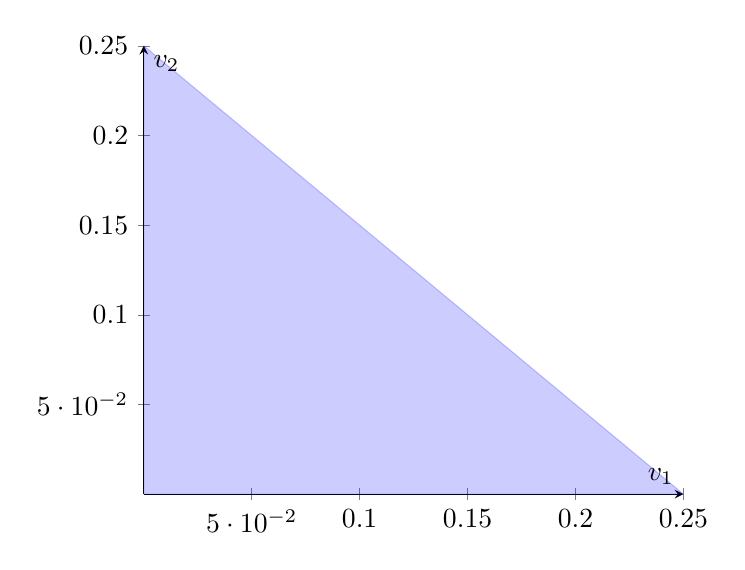
\begin{tikzpicture}
				\begin{axis}[
					xmin=0, xmax=0.25, xlabel=$v_1$,
					ymin=0, ymax=0.25, ylabel=$v_2$,
					samples=400,
					axis x line=middle,
					axis y line=middle,
					domain=0:1,
					]
					\draw[blue, fill = blue, opacity = 0.2] (axis cs: 0,0) -- (axis cs: 0,0.25) -- (axis cs: 0.25,0) -- (axis cs: 0,0);
					
				\end{axis}
			\end{tikzpicture}
		\end{center}
		\item Solve $(1-q_1-q_2)q_1 = v_1$ and $(1-q_1-q_2)q_2 = v_2$ gives
		\begin{align}
			q_1 &= \frac{v_1 - v_1\sqrt{1-4(v_1+v_2)}}{2(v_1+v_2)} \notag \\
			q_2 &= \frac{v_2 - v_2\sqrt{1-4(v_1+v_2)}}{2(v_1+v_2)} \notag
		\end{align}
		\item Nash reversion:
		\begin{align}
			s_i(h) \begin{cases}
				q_i(v) &\text{no deviation in }h \\
				\frac{1}{3} &\text{other}
			\end{cases} \notag
		\end{align}
		The upper bound for deviation is $\frac{1}{4}$. This leads to
		\begin{align}
			(1-\delta)\frac{1}{4} + (1-\delta)\sum_{t=1}^{\infty}\delta^t\frac{1}{9} &\le (1-\delta)\sum_{t=0}^\infty \delta^t v_i \notag \notag \\
			\delta &\ge \frac{\frac{1}{4}-v_1}{\frac{1}{4}-\frac{1}{9}} \notag
		\end{align}
		\item Yes because both $v_1$ are below $\frac{1}{4}$.
		\item No because $\frac{1}{12} < \frac{1}{3}$.
	\end{enumerate}

	\section*{Task 2: Cournot with Incomplete Information about Costs}
	\begin{enumerate}[label=(\alph*)]
		\item Maximizing $(1-q_1-q_2)q_1 - cq_1$ gives 
		\begin{align}
			q_1 &= \frac{1}{3} - \frac{2c_1}{3} + \frac{c_2}{3} \notag \\
			q_2 &= \frac{1}{3} - \frac{2c_2}{3} + \frac{c_1}{3} \notag
		\end{align}
		This results in $\left(\frac{1}{3},\frac{1}{3}\right)$.
		\item $\left(\frac{1}{4},\frac{1}{4}\right)$
		\item $\left(\frac{1}{6},\frac{5}{12}\right)$
		\item Maximizing expected utility gives
		\begin{align}
			q_1(0) &= \frac{1-pq_2(0) - (1-p)q_2(0.25)}{2} \notag \\
			q_1(0.25) &= \frac{\frac{3}{4}-pq_2(0) - (1-p)q_2(0.25)}{2} \notag
		\end{align}
		Same for player 2.
		\begin{align}
			q(0) &= \frac{9-p}{24} \notag \\
			q(0.25) &= \frac{6-p}{24} \notag
		\end{align}
		\item Beliefs are correlated, so $\mathbb{P}(c_2 = 0.25\mid c_1 = 0.25) = \mathbb{P}(c_2 = 0\mid c_1 = 0) = 2p$ and $\mathbb{P}(c_2 = 0.25 \mid c_1 = 0) = \mathbb{P}(c_2 = 0\mid c_1 = 0.25) = 1-2p$. This leads to
		\begin{align}
			q(0) &= \frac{14p+5}{12(4p+1)}\notag \\
			q(0.25) &= \frac{7p+1}{6(4p+1)} \notag
		\end{align}
		\item If $p=0.5$ we know the production costs of our opponent.
	\end{enumerate}

\end{document}